\documentclass[border=10pt]{standalone}
\usepackage[svgnames]{xcolor}
\usepackage{amsmath}
\usepackage{pgfplots}
\pgfplotsset{compat=newest}
\usepackage[sfdefault]{FiraSans}
\usepackage{FiraMono}
\renewcommand*\familydefault{\sfdefault}
\begin{document}
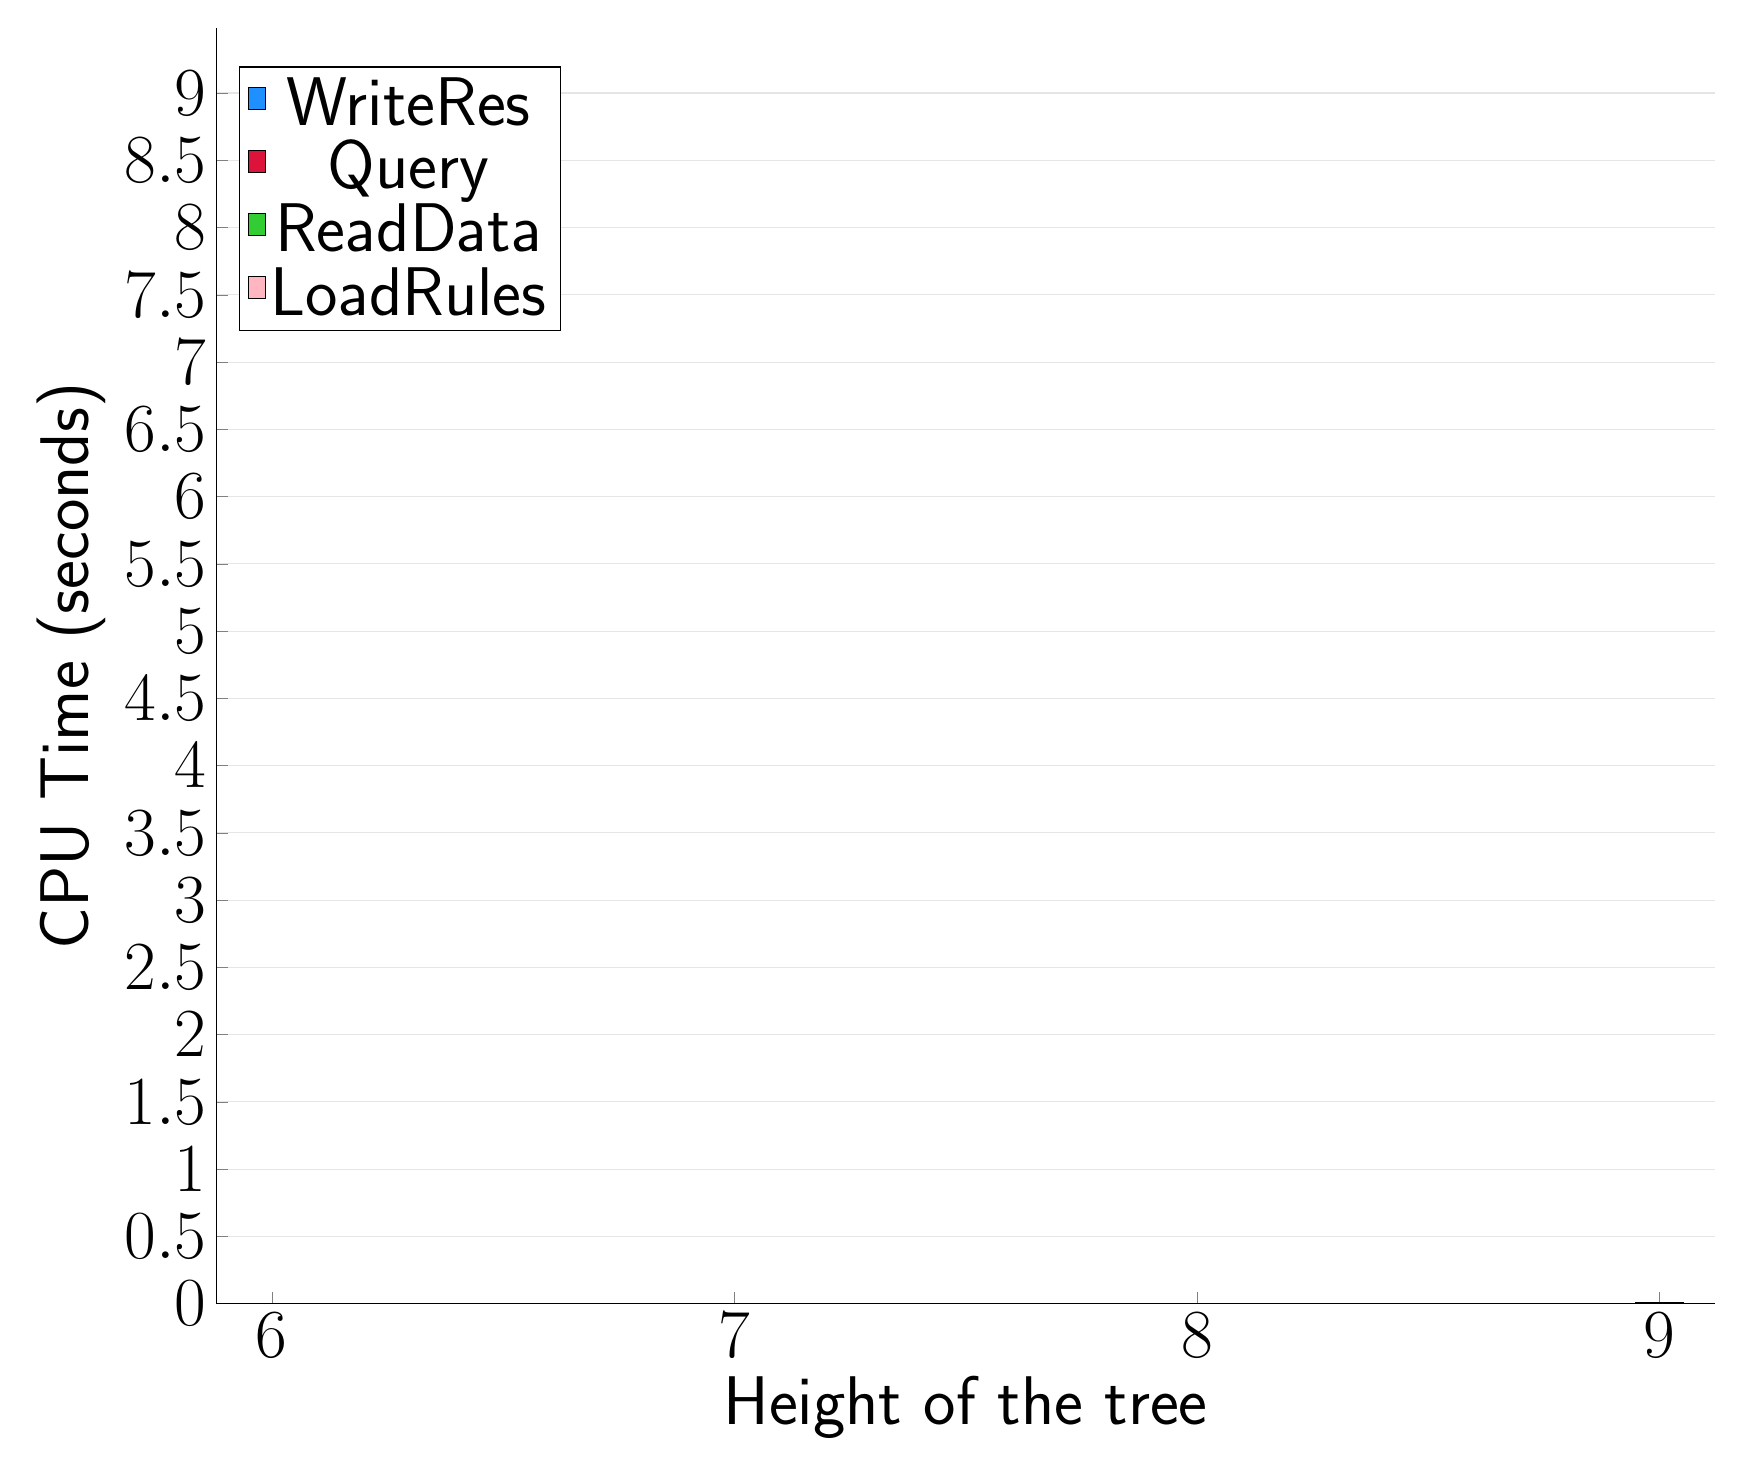
\begin{tikzpicture}
\begin{axis}[
   ybar stacked,
   width=1.7\textwidth,
   bar width=0.6cm,
   ymajorgrids, tick align=inside,
   major grid style={draw=gray!20},
   xtick=data,
   ymin=0, ymax=9.482,
   axis x line*=bottom,
   axis y line*=left,
   enlarge x limits=0.04,
   legend style={
       at={(0.23, 0.97)},
       anchor=north east,
       legend columns=1,
       font=\Huge,
   },
   ylabel={CPU Time (seconds)},
   xlabel={Height of the tree},
   label style={font=\Huge},
   tick label style={font=\Huge},
]
\addlegendimage{fill=DodgerBlue, draw=black, line width=0.2pt}
\addlegendentry{WriteRes}
\addlegendimage{fill=Crimson, draw=black, line width=0.2pt}
\addlegendentry{Query}
\addlegendimage{fill=LimeGreen, draw=black, line width=0.2pt}
\addlegendentry{ReadData}
\addlegendimage{fill=LightPink, draw=black, line width=0.2pt}
\addlegendentry{LoadRules}
\addplot +[fill=LightPink, draw=black, line width=0.55pt] coordinates {
(6, 0.0005593999999999997)
(7, 0.0005557999999999997)
(8, 0.000554)
(8, 0.0005533999999999998)
(8, 0.0005583999999999996)
(9, 0.0005496000000000001)
(9, 0.0005589999999999998)
(9, 0.0005527999999999998)
(9, 0.0005501999999999998)
(9, 0.0005510000000000002)
};
\addplot +[fill=LimeGreen, draw=black, line width=0.55pt] coordinates {
(6, 0.0001684000000000002)
(7, 0.0002196)
(8, 0.00031659999999999935)
(8, 0.0003245999999999998)
(8, 0.00032080000000000037)
(9, 0.0005143999999999997)
(9, 0.0005178000000000003)
(9, 0.0005141999999999998)
(9, 0.0005209999999999998)
(9, 0.0005191999999999998)
};
\addplot +[fill=Crimson, draw=black, line width=0.55pt] coordinates {
(6, 7.400000000000009e-05)
(7, 0.0001774000000000002)
(8, 0.00045620000000000003)
(8, 0.0004465999999999998)
(8, 0.0004416)
(9, 0.0011178000000000002)
(9, 0.0011052)
(9, 0.0011094000000000002)
(9, 0.0011098)
(9, 0.0011152)
};
\addplot +[fill=DodgerBlue, draw=black, line width=0.55pt] coordinates {
(6, 0.0002671999999999997)
(7, 0.0005975999999999993)
(8, 0.0012888)
(8, 0.0012970000000000002)
(8, 0.0013004)
(9, 0.0029424)
(9, 0.0029594)
(9, 0.0029584)
(9, 0.0030053999999999997)
(9, 0.0029820000000000003)
};
\end{axis}
\end{tikzpicture}

\end{document}
